\documentclass{standalone}
\usepackage{tikz}
\usetikzlibrary{patterns, positioning}


\begin{document}
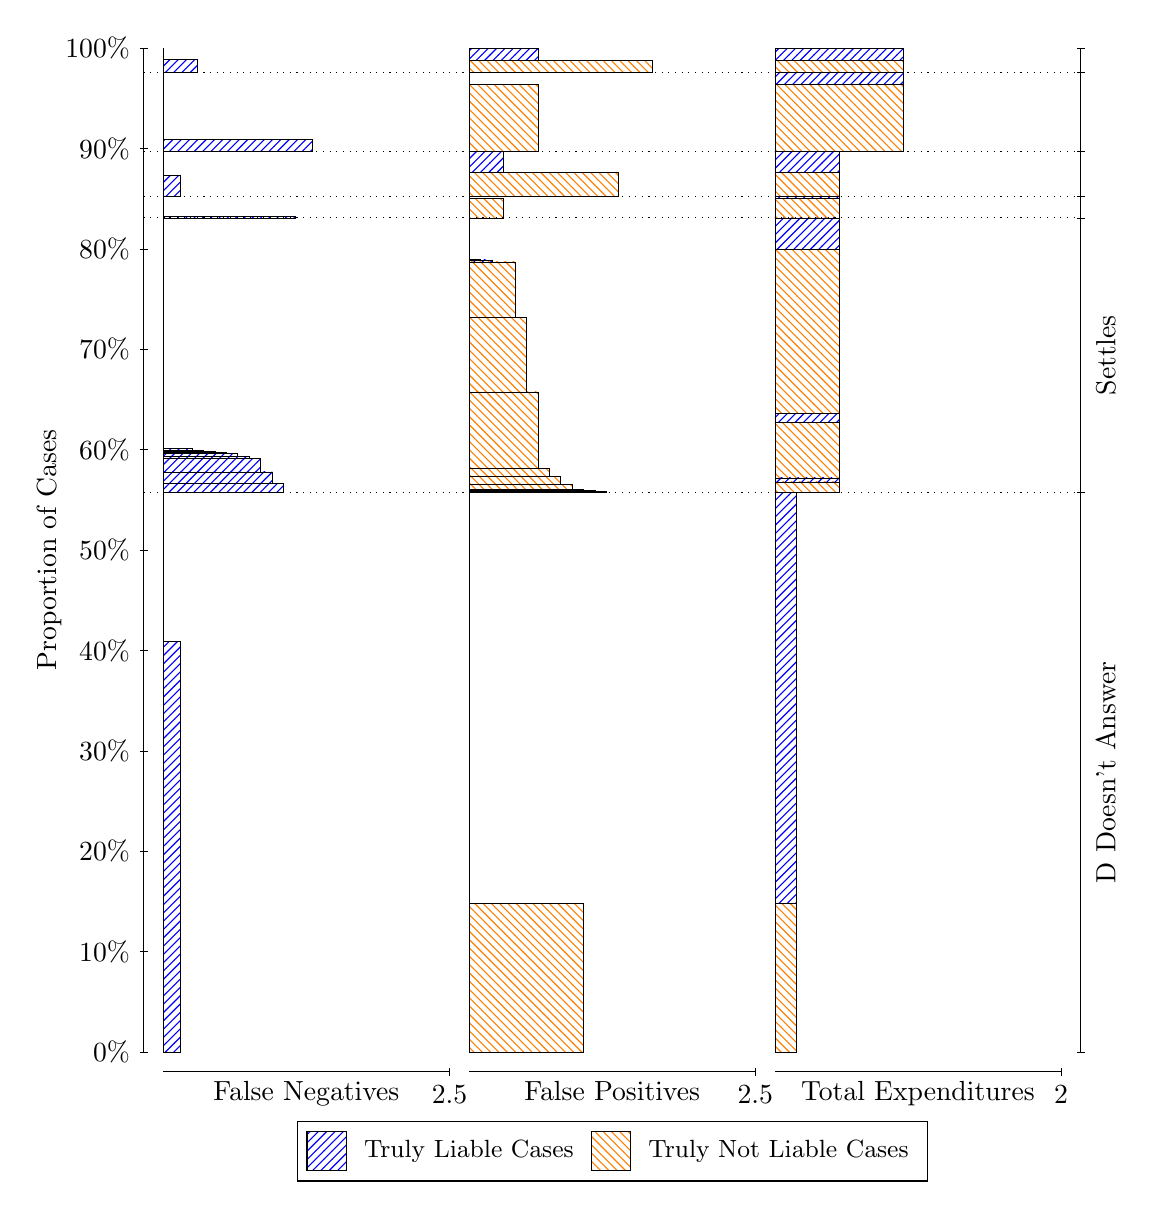
\begin{tikzpicture}
\draw[black, very thin] (1.5,1.75) -- (1.5,14.5);
\node[rotate=90, text=black, anchor=center] at (0.3, 8.125) {Proportion of Cases};
\draw[black, very thin] (1.45,1.75) -- (1.55,1.75);
\node[text=black, anchor=east] at (1.45, 1.75) {0\%};
\draw[black, very thin] (1.45,3.025) -- (1.55,3.025);
\node[text=black, anchor=east] at (1.45, 3.025) {10\%};
\draw[black, very thin] (1.45,4.3) -- (1.55,4.3);
\node[text=black, anchor=east] at (1.45, 4.3) {20\%};
\draw[black, very thin] (1.45,5.575) -- (1.55,5.575);
\node[text=black, anchor=east] at (1.45, 5.575) {30\%};
\draw[black, very thin] (1.45,6.85) -- (1.55,6.85);
\node[text=black, anchor=east] at (1.45, 6.85) {40\%};
\draw[black, very thin] (1.45,8.125) -- (1.55,8.125);
\node[text=black, anchor=east] at (1.45, 8.125) {50\%};
\draw[black, very thin] (1.45,9.4) -- (1.55,9.4);
\node[text=black, anchor=east] at (1.45, 9.4) {60\%};
\draw[black, very thin] (1.45,10.675) -- (1.55,10.675);
\node[text=black, anchor=east] at (1.45, 10.675) {70\%};
\draw[black, very thin] (1.45,11.95) -- (1.55,11.95);
\node[text=black, anchor=east] at (1.45, 11.95) {80\%};
\draw[black, very thin] (1.45,13.225) -- (1.55,13.225);
\node[text=black, anchor=east] at (1.45, 13.225) {90\%};
\draw[black, very thin] (1.45,14.5) -- (1.55,14.5);
\node[text=black, anchor=east] at (1.45, 14.5) {100\%};

\draw[black, very thin] (13.4,1.75) -- (13.4,14.5);
\draw[black, very thin] (13.35,1.75) -- (13.45,1.75);
\node[anchor=west] at (13.35, 1.75) {};
\draw[black, very thin] (13.35,8.8535) -- (13.45,8.8535);
\node[anchor=west] at (13.35, 8.8535) {};
\draw[black, very thin] (13.35,12.343) -- (13.45,12.343);
\node[anchor=west] at (13.35, 12.343) {};
\draw[black, very thin] (13.35,12.612) -- (13.45,12.612);
\node[anchor=west] at (13.35, 12.612) {};
\draw[black, very thin] (13.35,13.19) -- (13.45,13.19);
\node[anchor=west] at (13.35, 13.19) {};
\draw[black, very thin] (13.35,14.193) -- (13.45,14.193);
\node[anchor=west] at (13.35, 14.193) {};
\draw[black, very thin] (13.35,14.5) -- (13.45,14.5);
\node[anchor=west] at (13.35, 14.5) {};

\draw[black, very thin, pattern color=blue, pattern=north east lines] (1.75,1.75) rectangle (1.968,6.9674);
\draw[black, very thin, pattern color=orange, pattern=north west lines] (1.75,6.9674) rectangle (1.75,8.8535);
\draw[black, very thin, pattern color=blue, pattern=north east lines] (1.75,8.8535) rectangle (3.276,8.9672);
\draw[black, very thin, pattern color=blue, pattern=north east lines] (1.75,8.9672) rectangle (3.1307,9.1161);
\draw[black, very thin, pattern color=blue, pattern=north east lines] (1.75,9.1161) rectangle (2.9853,9.2878);
\draw[black, very thin, pattern color=blue, pattern=north east lines] (1.75,9.2878) rectangle (2.84,9.3177);
\draw[black, very thin, pattern color=blue, pattern=north east lines] (1.75,9.3177) rectangle (2.6947,9.3503);
\draw[black, very thin, pattern color=blue, pattern=north east lines] (1.75,9.3503) rectangle (2.5493,9.3685);
\draw[black, very thin, pattern color=blue, pattern=north east lines] (1.75,9.3685) rectangle (2.404,9.3785);
\draw[black, very thin, pattern color=blue, pattern=north east lines] (1.75,9.3785) rectangle (2.2587,9.3862);
\draw[black, very thin, pattern color=blue, pattern=north east lines] (1.75,9.3862) rectangle (2.1133,9.4129);
\draw[black, very thin, pattern color=orange, pattern=north west lines] (1.75,9.4129) rectangle (1.75,12.343);
\draw[black, very thin, pattern color=blue, pattern=north east lines] (1.75,12.343) rectangle (3.4213,12.363);
\draw[black, very thin, pattern color=orange, pattern=north west lines] (1.75,12.363) rectangle (1.75,12.612);
\draw[black, very thin, pattern color=blue, pattern=north east lines] (1.75,12.612) rectangle (1.968,12.879);
\draw[black, very thin, pattern color=orange, pattern=north west lines] (1.75,12.879) rectangle (1.75,13.19);
\draw[black, very thin, pattern color=blue, pattern=north east lines] (1.75,13.19) rectangle (3.6393,13.342);
\draw[black, very thin, pattern color=orange, pattern=north west lines] (1.75,13.342) rectangle (1.75,14.193);
\draw[black, very thin, pattern color=blue, pattern=north east lines] (1.75,14.193) rectangle (2.186,14.352);
\draw[black, very thin, pattern color=orange, pattern=north west lines] (1.75,14.352) rectangle (1.75,14.5);
\draw[black, very thin, pattern color=orange, pattern=north west lines] (5.6333,1.75) rectangle (7.0867,3.6361);
\draw[black, very thin, pattern color=blue, pattern=north east lines] (5.6333,3.6361) rectangle (5.6333,8.8535);
\draw[black, very thin, pattern color=orange, pattern=north west lines] (5.6333,8.8535) rectangle (7.3773,8.8701);
\draw[black, very thin, pattern color=orange, pattern=north west lines] (5.6333,8.8701) rectangle (7.232,8.881);
\draw[black, very thin, pattern color=orange, pattern=north west lines] (5.6333,8.881) rectangle (7.0867,8.8982);
\draw[black, very thin, pattern color=orange, pattern=north west lines] (5.6333,8.8982) rectangle (6.9413,8.9559);
\draw[black, very thin, pattern color=orange, pattern=north west lines] (5.6333,8.9559) rectangle (6.796,9.0645);
\draw[black, very thin, pattern color=orange, pattern=north west lines] (5.6333,9.0645) rectangle (6.6507,9.1661);
\draw[black, very thin, pattern color=orange, pattern=north west lines] (5.6333,9.1661) rectangle (6.5053,10.134);
\draw[black, very thin, pattern color=orange, pattern=north west lines] (5.6333,10.134) rectangle (6.36,11.077);
\draw[black, very thin, pattern color=orange, pattern=north west lines] (5.6333,11.077) rectangle (6.2147,11.783);
\draw[black, very thin, pattern color=blue, pattern=north east lines] (5.6333,11.783) rectangle (5.924,11.81);
\draw[black, very thin, pattern color=blue, pattern=north east lines] (5.6333,11.81) rectangle (5.7787,11.818);
\draw[black, very thin, pattern color=blue, pattern=north east lines] (5.6333,11.818) rectangle (5.6333,12.343);
\draw[black, very thin, pattern color=orange, pattern=north west lines] (5.6333,12.343) rectangle (6.0693,12.591);
\draw[black, very thin, pattern color=blue, pattern=north east lines] (5.6333,12.591) rectangle (5.6333,12.612);
\draw[black, very thin, pattern color=orange, pattern=north west lines] (5.6333,12.612) rectangle (7.5227,12.923);
\draw[black, very thin, pattern color=blue, pattern=north east lines] (5.6333,12.923) rectangle (6.0693,13.19);
\draw[black, very thin, pattern color=orange, pattern=north west lines] (5.6333,13.19) rectangle (6.5053,14.042);
\draw[black, very thin, pattern color=blue, pattern=north east lines] (5.6333,14.042) rectangle (5.6333,14.193);
\draw[black, very thin, pattern color=orange, pattern=north west lines] (5.6333,14.193) rectangle (7.9587,14.341);
\draw[black, very thin, pattern color=blue, pattern=north east lines] (5.6333,14.341) rectangle (6.5053,14.5);
\draw[black, very thin, pattern color=orange, pattern=north west lines] (9.5167,1.75) rectangle (9.7892,3.6361);
\draw[black, very thin, pattern color=blue, pattern=north east lines] (9.5167,3.6361) rectangle (9.7892,8.8535);
\draw[black, very thin, pattern color=orange, pattern=north west lines] (9.5167,8.8535) rectangle (10.334,8.9903);
\draw[black, very thin, pattern color=blue, pattern=north east lines] (9.5167,8.9903) rectangle (10.334,9.0405);
\draw[black, very thin, pattern color=orange, pattern=north west lines] (9.5167,9.0405) rectangle (10.334,9.7468);
\draw[black, very thin, pattern color=blue, pattern=north east lines] (9.5167,9.7468) rectangle (10.334,9.8604);
\draw[black, very thin, pattern color=orange, pattern=north west lines] (9.5167,9.8604) rectangle (10.334,11.947);
\draw[black, very thin, pattern color=blue, pattern=north east lines] (9.5167,11.947) rectangle (10.334,12.343);
\draw[black, very thin, pattern color=orange, pattern=north west lines] (9.5167,12.343) rectangle (10.334,12.591);
\draw[black, very thin, pattern color=blue, pattern=north east lines] (9.5167,12.591) rectangle (10.334,12.612);
\draw[black, very thin, pattern color=orange, pattern=north west lines] (9.5167,12.612) rectangle (10.334,12.923);
\draw[black, very thin, pattern color=blue, pattern=north east lines] (9.5167,12.923) rectangle (10.334,13.19);
\draw[black, very thin, pattern color=orange, pattern=north west lines] (9.5167,13.19) rectangle (11.152,14.042);
\draw[black, very thin, pattern color=blue, pattern=north east lines] (9.5167,14.042) rectangle (11.152,14.193);
\draw[black, very thin, pattern color=orange, pattern=north west lines] (9.5167,14.193) rectangle (11.152,14.341);
\draw[black, very thin, pattern color=blue, pattern=north east lines] (9.5167,14.341) rectangle (11.152,14.5);
\draw[black, dotted] (1.5,8.8535) -- (13.4,8.8535);
\draw[black, dotted] (1.5,12.343) -- (13.4,12.343);
\draw[black, dotted] (1.5,12.612) -- (13.4,12.612);
\draw[black, dotted] (1.5,13.19) -- (13.4,13.19);
\draw[black, dotted] (1.5,14.193) -- (13.4,14.193);
\draw[black, very thin] (1.75,1.5) -- (5.3833,1.5);
\node[text=black, anchor=north] at (3.5667, 1.5) {False Negatives};
\draw[black, very thin] (5.3833,1.45) -- (5.3833,1.55);
\node[text=black, anchor=north] at (5.3833, 1.45) {2.5};

\draw[black, very thin] (5.6333,1.5) -- (9.2667,1.5);
\node[text=black, anchor=north] at (7.45, 1.5) {False Positives};
\draw[black, very thin] (9.2667,1.45) -- (9.2667,1.55);
\node[text=black, anchor=north] at (9.2667, 1.45) {2.5};

\draw[black, very thin] (9.5167,1.5) -- (13.15,1.5);
\node[text=black, anchor=north] at (11.333, 1.5) {Total Expenditures};
\draw[black, very thin] (13.15,1.45) -- (13.15,1.55);
\node[text=black, anchor=north] at (13.15, 1.45) {2};

\node[text=black, centered, rotate=90] at (13.72, 5.3018) {D Doesn't Answer};
\node[text=black, centered, rotate=90] at (13.72, 10.598) {Settles};





\draw (7.449999999999999,1.5) node[draw=none] (baseCoordinate) {};
\begin{scope}[align=center]
        \matrix[scale=0.5, draw=black, below=0.5cm of baseCoordinate, nodes={draw}, column sep=0.1cm]{
            \node[rectangle, draw, minimum width=0.5cm, minimum height=0.5cm, pattern color=blue, pattern=north east lines] {}; &
            \node[draw=none, font=\small, text=black] (B) {Truly Liable Cases}; &
            \node[rectangle, draw, minimum width=0.5cm, minimum height=0.5cm, pattern color=orange, pattern=north west lines] {}; &
            \node[draw=none, font=\small, text=black] (B) {Truly Not Liable Cases}; \\
            };
\end{scope}

\end{tikzpicture}
\end{document}